\documentclass[landscape]{article}
\usepackage{graphicx,color,amssymb}
%% \usepackage{bm}
\pagestyle{plain}
\oddsidemargin  -0.5 in
\evensidemargin -0.5 in
\headheight     0 in
\topmargin      -1 in
\textheight     7.5 in
\textwidth      10 in
\newenvironment{slide}[1][ ]{\mbox{\bf #1 } \vfill}{\vfill \mbox{ } \pagebreak}
\begin{document}
\huge \sf \boldmath
\renewcommand{\labelitemi}{-}
\setlength{\parindent}{0 cm}

\begin{slide}
  \begin{center}
    \Huge Di-Electron Widths of $\Upsilon(1S)$, $\Upsilon(2S)$, and $\Upsilon(3S)$ \\
    as a Test of Lattice QCD

    \vspace{2 cm}
    Jim Pivarski

    \vspace{1 cm}
    CLEO Collaboration
  \end{center}
\end{slide}

\begin{slide}[Definition and Motivation]

Di-electron width $\Gamma_{ee} = \mathcal{B}_{ee} \Gamma$

\vfill

Goal: precisely measure $\Gamma_{ee}$ of $\Upsilon(1S)$,
$\Upsilon(2S)$, and $\Upsilon(3S)$

\vfill

Why?

\begin{center}
  \begin{center}
    \begin{tabular}{c p{1 cm} c}
      $\Gamma_{ee}$ & & ${f_B}^2$ \\
      \includegraphics[width=0.4\linewidth]{diagram_gamee2} & &
      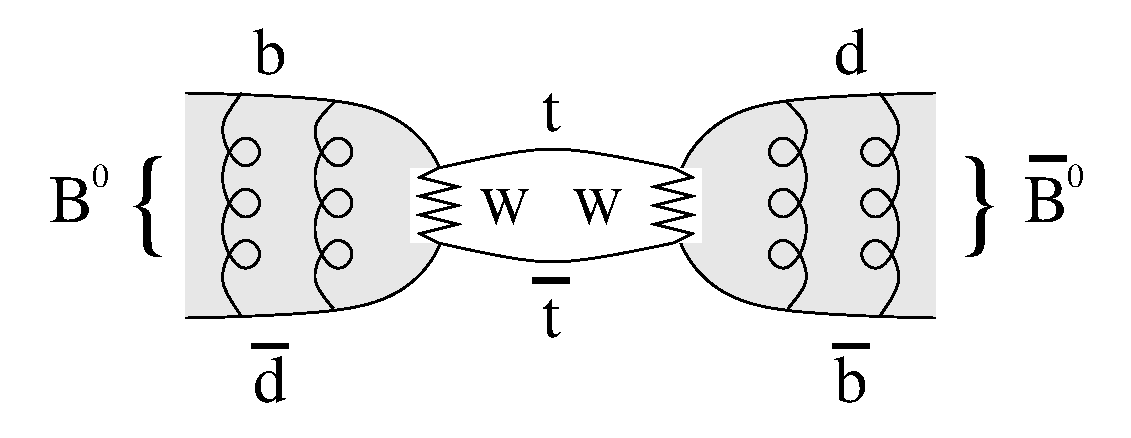
\includegraphics[width=0.4\linewidth]{diagram_bmixing}
    \end{tabular}
  \end{center}

  \vspace{0.5 cm}
  Treated similarly in Lattice QCD

\end{center}

\vfill

Lattice QCD calculations of $\Gamma_{ee}$ and $f_B$ are both in progress

\vfill

$\Gamma_{ee}$ gives us three high-precision tests of Lattice QCD in a
decay related to $B$ mixing

\end{slide}

\begin{slide}[Experimental Technique]

Use the time-reversed process: production cross-section of $\Upsilon$ from $e^+e^-$

\vspace{0.5 cm}

\[   \Gamma_{ee} = \frac{{M_\Upsilon}^2}{6\pi^2} \int \sigma(e^+e^- \to \Upsilon) \, dE \]

\vspace{1 cm}

Resonances scanned by Cornell Electron Storage Ring (Nov 2001 -- Aug 2002)

\vspace{0.5 cm}

\begin{center}
  \begin{tabular}{p{0.45\linewidth} p{0.5 cm} p{0.45\linewidth}}
    \begin{minipage}{\linewidth}
      \begin{center}
	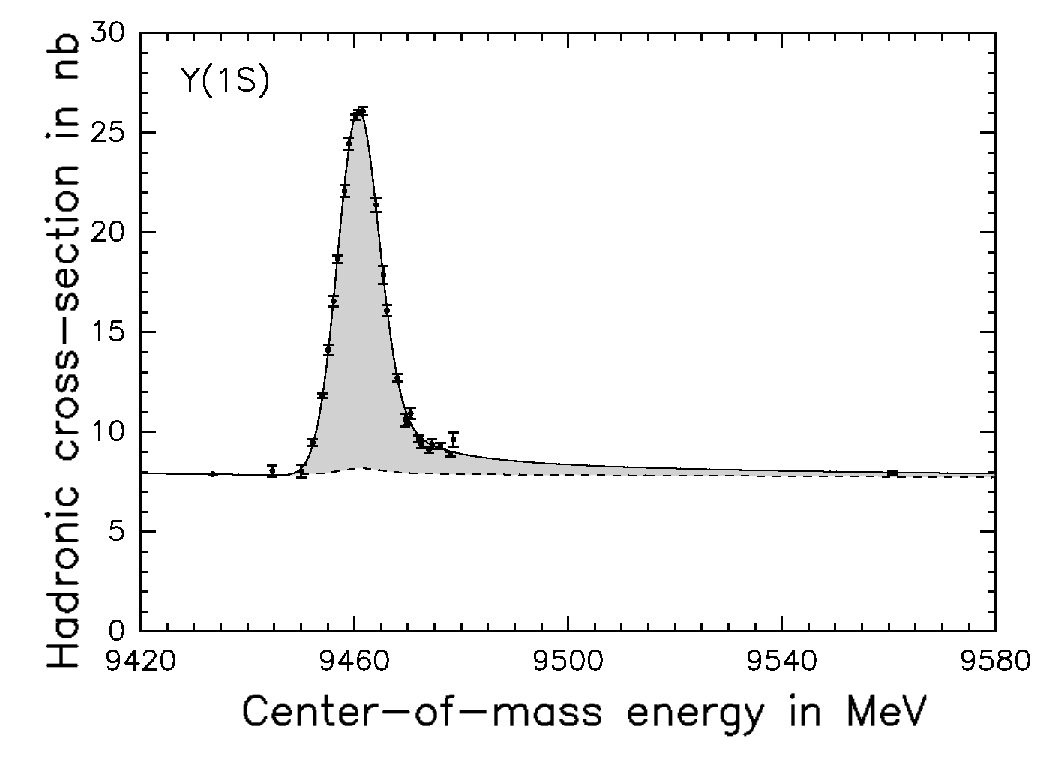
\includegraphics[width=\linewidth]{prettied_individual07_noinset_1s}
      \end{center}
    \end{minipage} & &
    \begin{minipage}{\linewidth}
	Data collected by CLEO-III detector:

	\begin{center}
	  \renewcommand{\arraystretch}{1.25}
	  \begin{tabular}{c c c}
	    & scan & off-resonance \\\hline
	    $\Upsilon(1S)$ & 0.10 fb$^{-1}$ & 0.18 fb$^{-1}$ \\
	    $\Upsilon(2S)$ & 0.06 fb$^{-1}$ & 0.44 fb$^{-1}$ \\
	    $\Upsilon(3S)$ & 0.10 fb$^{-1}$ & 0.16 fb$^{-1}$ \\
	  \end{tabular}
	\end{center}
	\vspace{0.5 cm}

	50 times Novosibirsk 1996
	
    \end{minipage}
  \end{tabular}
\end{center}

\vspace{1 cm}

All but a well-measured fraction of $\Upsilon$ decays are hadronic

\vspace{0.5 cm}

Select hadronic final states inclusively

\vspace{-1 cm}

\end{slide}

\begin{slide}[Hadronic Backgrounds]

\vspace{0.5 cm}
Most are effectively subtracted by including a $1/s$ term in the fit

\vspace{0.5 cm}
The rest are very small corrections

\vspace{0.5 cm}

\begin{center}
  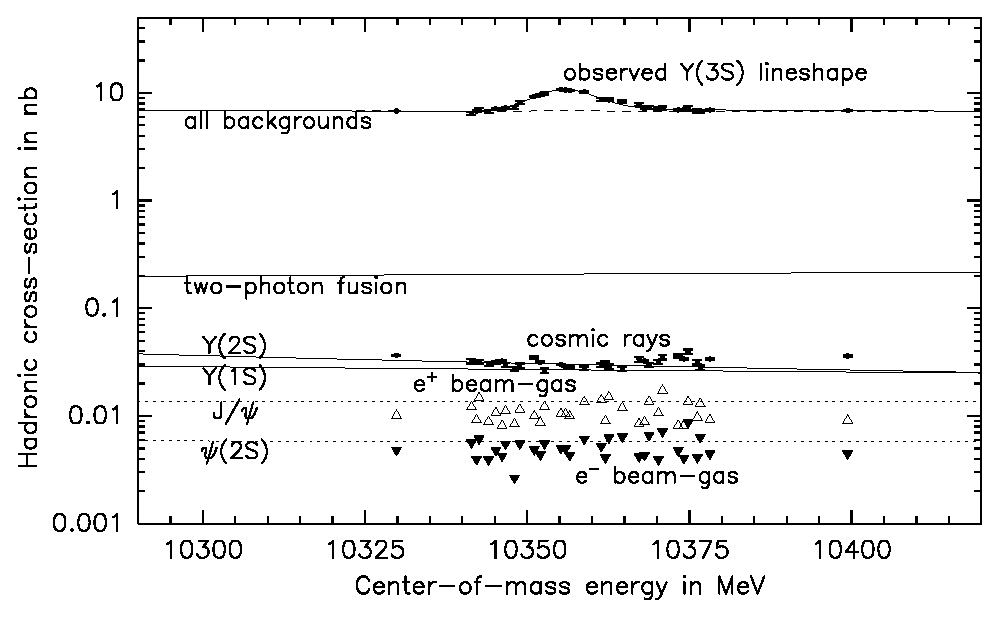
\includegraphics[width=0.9\linewidth]{../notau_backgrounds_6}
\end{center}

\vspace{-1 cm}

\end{slide}

\begin{slide}[Hadronic Efficiency]

\renewcommand{\labelitemi}{}

\vspace{0.5 cm}

  Model-independent, data-based method for measuring hadronic
    efficiency:

\vspace{0.5 cm}

    \begin{tabular}{p{0.6\linewidth} c p{0.38\linewidth}}
      \hspace{-1 cm}\begin{minipage}{\linewidth}
	\vspace{1 cm}
        \begin{itemize}\setlength{\itemsep}{0.7 cm}

          \item Select \mbox{$\Upsilon(2S) \to \pi^+ \pi^- \ \Upsilon(1S)$} \\ \mbox{ } \hfill based on $\pi^+ \pi^-$ only (1.3 fb$^{-1}$)

          \item Set of recoiling $\Upsilon(1S)$ events 
	    includes all decays, \\ \mbox{ } \hfill even undetectable modes

          \item \#pass/\#total = $\epsilon_{1S}$ = (97.8 $\pm$ 0.5)\%

        \end{itemize}
      \end{minipage} & & \begin{minipage}{\linewidth}
	\vspace{0.5 cm}
	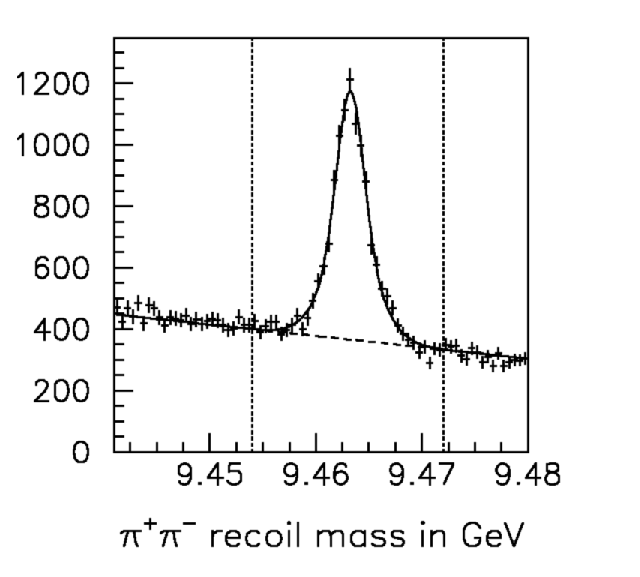
\includegraphics[width=\linewidth]{prettied_plenary_justpipimass}

	\vspace{-0.75 cm}
      \end{minipage}
    \end{tabular}

\vspace{1.5 cm} $\Upsilon(2S)$ and $\Upsilon(3S)$ inherit this efficiency with (largest) correction for
\[ \mbox{\hspace{4 cm}} \Upsilon' \to X \Upsilon \to X \ell^+\ell^- \mbox{ \hspace{1 cm} ($\ell$ is $e$ or $\mu$)}\]

\vspace{0.75 cm} $X \ell^+\ell^-$ branching fractions measured in data (1.58 $\pm$ 0.15)\% and (1.34 $\pm$ 0.15)\%

\vspace{1 cm} $\epsilon_{2S}$ = (95.8 $\pm$ 0.6)\% and $\epsilon_{3S}$ = (96.0 $\pm$ 0.6)\%

\vspace{-1 cm}

\end{slide}

\begin{slide}[Integrated Luminosity]

\vspace{0.4 cm} We need integrated luminosity for every cross-section measurement:

\[ \sigma_i = \mbox{(\# hadrons)}_i / \mbox{(integrated luminosity)}_i \]

\vspace{0.7 cm}
Count $e^+e^- \to \gamma\gamma$ events at each energy point ($\Upsilon \not\to \gamma\gamma$)

\vspace{0.8 cm} Normalize to physical units (nb$^{-1}$)

\vspace{0.5 cm}
\begin{center}
  \includegraphics[width=0.8\linewidth]{panic_lumi}
\end{center}

\end{slide}

\begin{slide}[Beam Energy Measurement]

\begin{tabular}{p{0.6\linewidth} p{0.38\linewidth}}
  \begin{minipage}{\linewidth}
    \begin{minipage}{0.9\linewidth}

      Obtain $E_{beam}$ from dipole $\vec{B}$ measurement

      \vspace{0.5 cm}
      \hspace{1 cm} (sensitive to position of probe)

      \vspace{1.5 cm}
      Collect scan data in short, independent trials

      \vspace{0.5 cm}
      \hspace{1 cm} $\rightarrow$ $E_{beam}$ is reproducible to $\sim$ 0.5 MeV

      \hfill between mini-scans

      \vspace{1.5 cm}
      Alternate scan order above and below peak

      \vspace{1.5 cm}
      Repeat point of highest slope

      \vspace{0.5 cm}
      \hspace{1 cm} $\rightarrow$ $E_{beam}$ is reproducible to $\lesssim$ 0.07 MeV

      \mbox{ } \hfill during a mini-scan

      \vspace{0.2 cm}
      \hspace{1 cm} $\rightarrow$ 0.2\% uncertainty in $\Gamma_{ee}$

    \end{minipage}

  \end{minipage} &
  \begin{minipage}{\linewidth}
    \includegraphics[width=\linewidth]{../plenary_fitorder}
  \end{minipage}
\end{tabular}

\end{slide}

\begin{slide}[Fit Results]

\vspace{0.5 cm}
\begin{center}
  \includegraphics[width=\linewidth]{xfiged_three_resonances_inset_squat2}
\end{center}
\vspace{-1 cm}

\end{slide}

\begin{slide}[Summary of Uncertainties]

Preliminary Results

\vspace{1 cm}
\begin{center}
  \renewcommand{\arraystretch}{1.5}
  \begin{tabular}{l c c c}
    Contribution to $\Gamma_{ee}$ & \mbox{\hspace{0.75 cm}} $\Upsilon(1S)$ \mbox{\hspace{0.75 cm}} & \mbox{\hspace{0.75 cm}} $\Upsilon(2S)$ \mbox{\hspace{0.75 cm}} & \mbox{\hspace{0.75 cm}} $\Upsilon(3S)$ \mbox{\hspace{0.75 cm}} \\\hline
    Statistical$^*$               & {\color{red} 0.7\%}  & {\color{red} 1.6\%}  & {\color{red} 2.2\%} \\
    Correct for leptonic modes & 0.2\%  & 0.2\%  & 0.3\% \\
    Hadronic efficiency           & 0.5\%  & 0.6\%  & 0.7\% \\
    Luminosity calibration        & {\color{red} $\longleftarrow$} & {\color{red} 1.3\%}  & {\color{red} $\longrightarrow$} \\
    Cross-section stability       & 0.1\%  & 0.1\%  & 0.1\% \\
    Beam-energy stability         & 0.2\%  & 0.2\%  & 0.2\% \\
    Shape of the fit function     & 0.05\% & 0.06\% & 0.05\% \\\hline
    Total                         & {\color{red} 1.6\%}  & {\color{red} 2.2\%}  & {\color{red} 2.7\%} \\
  \end{tabular}
\end{center}

\vspace{1 cm}

\mbox{ }$^*$ Statistical uncertainty is dominated by $\gamma\gamma$ counting

\end{slide}

\begin{slide}[Preliminary Results]

\begin{center}
  \renewcommand{\arraystretch}{2}
  \begin{tabular}{c c c}
    Quantity & Value & \mbox{\hspace{0.5 cm}} Uncertainty \mbox{\hspace{0.5 cm}} \\ \hline
    $\Gamma_{ee}(1S)$ & \mbox{\hspace{0.5 cm}} 1.336 $\pm$ 0.009 $\pm$ 0.019 keV \mbox{\hspace{0.5 cm}} & {\color{red} 1.6\%} \\
    $\Gamma_{ee}(2S)$ & 0.616 $\pm$ 0.010 $\pm$ 0.009 keV & {\color{red} 2.2\%} \\
    $\Gamma_{ee}(3S)$ & 0.425 $\pm$ 0.009 $\pm$ 0.006 keV & {\color{red} 2.7\%} \\ \hline
    $\Gamma_{ee}(2S)$/$\Gamma_{ee}(1S)$ & 0.461 $\pm$ 0.008 $\pm$ 0.003 & {\color{red} 1.8\%} \\
    $\Gamma_{ee}(3S)$/$\Gamma_{ee}(1S)$ & 0.318 $\pm$ 0.007 $\pm$ 0.002 & {\color{red} 2.4\%} \\
    $\Gamma_{ee}(3S)$/$\Gamma_{ee}(2S)$ & 0.690 $\pm$ 0.019 $\pm$ 0.006 & {\color{red} 2.8\%} \\
  \end{tabular}
\end{center}

\end{slide}

\begin{slide}[Preliminary Results (keV)]

\begin{center}
  \vspace{1.5 cm}
  \includegraphics[width=0.95\linewidth, trim=0 0.5cm 0 1.8cm]{/home/mccann/monster_talk/pdgplots2}
\end{center}

\end{slide}

\begin{slide}[Preliminary Results (keV)]

\begin{center}
  \includegraphics[width=0.8\linewidth]{prettied-zoomed_pdgplots2}
\end{center}

\end{slide}

\begin{slide}[Comparison with Theory]

\vspace{0.5 cm}
Lattice calculation is still in progress, but ratio of $\Gamma_{ee}(2S)/\Gamma_{ee}(1S)$ may be compared

\vspace{0.5 cm}
Partial result is very sensitive to lattice spacing \hfill \fbox{\tt hep-lat/0507013}

\vspace{0.5 cm}
\begin{center}
  \includegraphics[width=0.6\linewidth]{/home/mccann/monster_talk/take_two/dependence}
\end{center}

\vspace{0.5 cm}
Consistent, but with 10\% uncertainty (due to extrapolation)

\vspace{0.5 cm}
Final lattice precision will be few percent in {\it ratios}

\vspace{-1 cm}

\end{slide}

\begin{slide}[Conclusions]

\renewcommand{\labelitemi}{}
\begin{itemize}\setlength{\itemsep}{1.5 cm}

  \item Very careful 1.5--3\% measurement of $\Gamma_{ee}$ and $\Gamma_{ee}$ ratios

  \item Final result will determine luminosity from $e^+e^-$, rather than $\gamma\gamma$

  \item Tight constraint on Lattice QCD, also a useful input for potential model fits

  \item With new $\mathcal{B}_{\mu\mu}$ from {\tt PRL 94, 012001} (2005),

\begin{center}
  \renewcommand{\arraystretch}{2}
  \begin{tabular}{c c c c}
    $\Gamma(1S)$ & \mbox{\hspace{0.5 cm}} 53.7 $\pm$ 1.7 keV \mbox{\hspace{0.5 cm}} & 3.2\% & \mbox{\hspace{0.5 cm}} (0.3 $\sigma$ above PDG) \mbox{\hspace{0.5 cm}} \\
    $\Gamma(2S)$ & 30.3 $\pm$ 1.4 keV & 4.5\% & (2.1 $\sigma$ below PDG) \\
    $\Gamma(3S)$ & 17.8 $\pm$ 1.0 keV & 5.8\% & (2.4 $\sigma$ below PDG)
  \end{tabular}
\end{center}

\end{itemize}

\end{slide}

%%     \includegraphics[width=0.6\linewidth]{../proceedings_cartoon}    
%% 	\includegraphics[width=\linewidth, bb=0 0 540 520]{../proceedings_cuts3}
%% 	\includegraphics[width=\linewidth]{../plenary_justpipimass}
%% 	  \includegraphics[width=0.7\linewidth]{../cascade_correction_white}
%% 	  \includegraphics[width=0.7\linewidth]{../cascade_correction_white}
%% 	\includegraphics[width=\linewidth]{../plenary_justpipimass}
%% 	  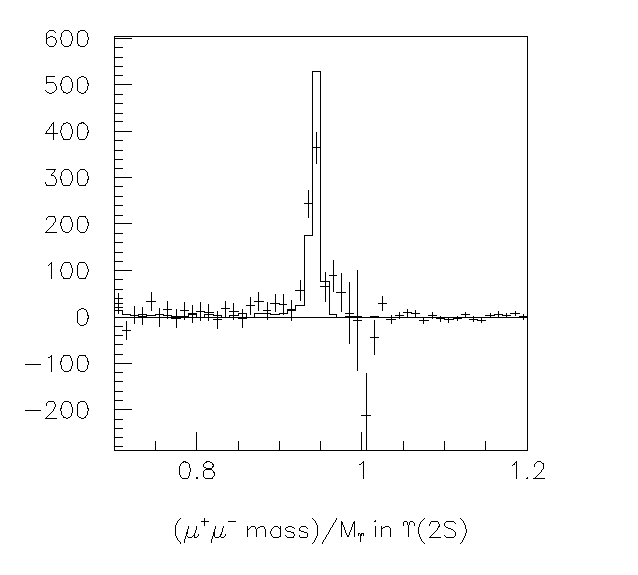
\includegraphics[width=0.7\linewidth]{../cascade_correction_2s}
%% 	  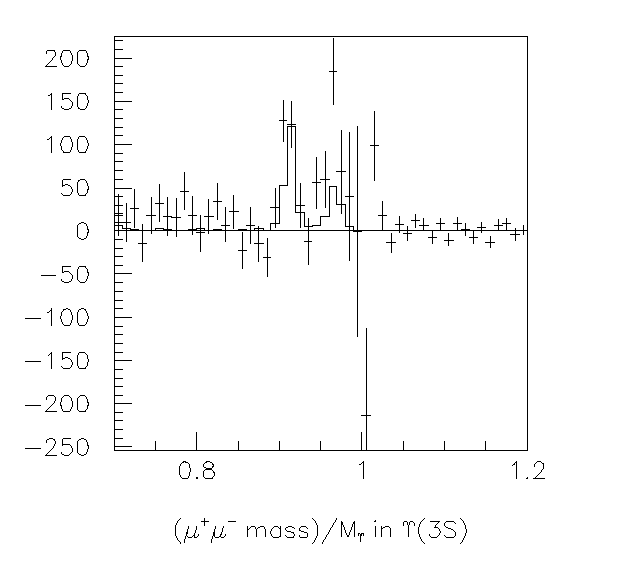
\includegraphics[width=0.7\linewidth]{../cascade_correction_3s}
%%     \includegraphics[width=0.9\linewidth]{../jed_backgrounds}
%%     \includegraphics[width=0.75\linewidth]{../plenary_lumi}
%%     \includegraphics[width=\linewidth]{stability}
%% 	\includegraphics[width=0.95\linewidth]{../proceedings_miscal_white}
%%       \includegraphics[width=\linewidth]{../plenary_fitorder}
%% 	\includegraphics[width=0.95\linewidth]{../proceedings_miscal}
%%       \includegraphics[width=\linewidth]{../plenary_fitorder}
%%       \includegraphics[width=\linewidth]{../individual_noinset_1s}
%%     \includegraphics[width=\linewidth]{../three_resonances_inset_squat2_nscans}
%%     \includegraphics[width=0.85\linewidth]{../plenary_pulls1}
%%     \includegraphics[width=0.85\linewidth]{../plenary_pulls2}
%%     \includegraphics[width=0.85\linewidth]{../plenary_pulls3}
%%     \includegraphics[width=0.9\linewidth]{pdgplots2}
%%     \includegraphics[width=\linewidth]{dependence}

\end{document}
